\chapter{History of Neural Networks}\label{ch_history}
\chapterauthor{Jeff Yoshimi}

% Consider separating second winter, and deep learning resurgence, even if the resulting sections are short, for a cleaner presentation.
% Can say more about the two resurgences.  Both involves more on learning intermediate reps in FF networks. Part of a narrative across chapters

This chapter briefly outlines the history of neural networks, including the pre-history of neural networks and cognitive science extending back to ancient Egypt. The theory of neural networks has many historical precedents, but emerged as an explicit mathematical and computational formalism in the mid 1900s, via the work of McCulloch and Pitts. The main events developed in the chapter are shown in Fig. \ref{timelineHistory}. 

\begin{figure}[h]
\centering
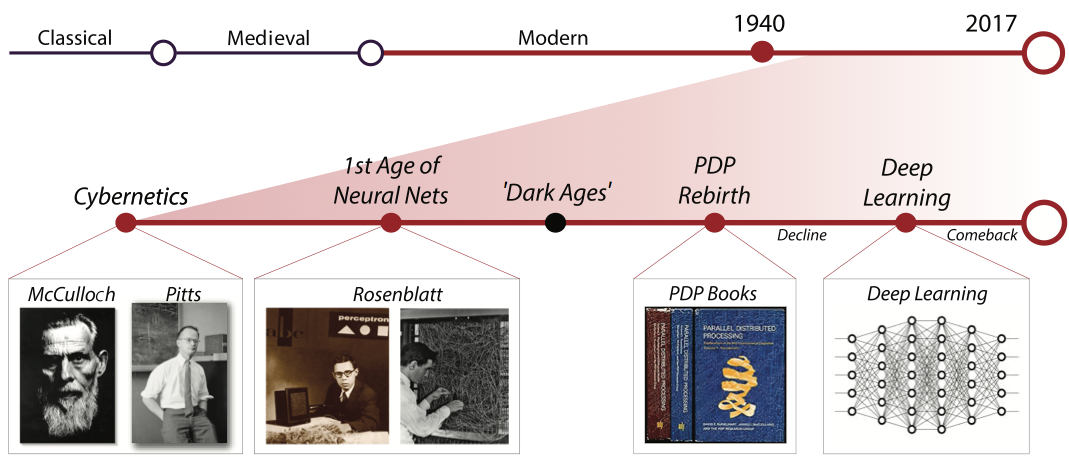
\includegraphics[width=0.8\textwidth]{images/historyTimeline.png}
\caption[Pamela Payne and Jeff Yoshimi.]{A timeline of the history of neural networks. The main history of neural networks runs from the mid 1940s to the present. We  also consider some of the pre-history of neural networks,  i.e. historical figures who linked the structure and dynamics of the mind with the structure and dynamics of the brain.}
\label{timelineHistory}
\end{figure}

\section{Pre-history}

Cognitive science, the interdisciplinary study of mind, has ancient roots. Documentation of the idea that the brain plays some role in controlling behavior goes back to an Egyptian papyrus that is over 3000 years old.\footnote{The papyrus can be viewed online; try searching for ``Smith papyrus''. Recent scholarship on the papyrus is collected in \cite{meltzer2014edwin}.} Hieroglyphics from the papyrus describing the gyrations of the brain are shown in Fig. \ref{papyrus}. 
% Source: https://www.princeton.edu/~cggross/Hist_Neurosci_Ency_neurosci.pdf

\begin{figure}[h]
\centering

\includegraphics[width=0.4\textwidth]{images/papyrus.png}
\caption[From \url{https://faculty.washington.edu/chudler/papy.html}]{Hieroglyphics describing the sulci and gyri of the brain.}
\label{papyrus}
\end{figure}

In Western philosophy and science, Plato, Aristotle, and other Greek philosophers had an interest in the structure of the human mind (or ``soul'') in relation to physical processes in the body.\footnote{I focus on Western roots of neural network theory, though there were precedents in other parts of the world, which I hope to add in future versions of this chapter. Currently, the literature is sparse. There is an expanding literature on the history of science globally (e.g \cite{selin2013encyclopaedia}), but there is not (as of 2017) much scholarship on the history of neuroscience, cognitive science, or psychology in Africa, Asia, India, Meso-America, the Middle East, and other regions whose historical documents contain relevant information. There is however, some literature on  Arabic and Islamic roots of neuroscience \cite{mohamed2008arab}.}  Plato and Aristotle both described the soul as a set of interacting faculties (in Plato: reason, spirit, and appetite), and both speculated about its physical basis. They disagreed  about whether the brain or heart is the physical basis of the soul (Aristotle thought the brain just cooled the blood), but by the end of the Classical period the dispute was resolved in favor of the brain \cite{finger2001origins}.

In the Medieval period, priests, physicians, and natural philosophers throughout Europe and the Middle East discussed cognition in relation to the brain. Cognition was thought to be based on the play of ``spirits'' or vapors in the ventricles of the brain \cite{finger2001origins}. Spirits originating in the senses were combined in the ``common sense'' and then purified, and mixed in higher ventricles. A typical diagram from the period is shown in figure \ref{medieval}. The ventricles are now believed to be shock-absorbers and chemical reservoirs. They are not thought to play a central functional role in cognition. However, the idea that sensory inputs to the brain are combined and refined in various ways persists in connectionist models.
% https://web.stanford.edu/class/history13/earlysciencelab/body/brainpages/brain.html   // Mention Avicenna here

\begin{figure}[h]
\centering
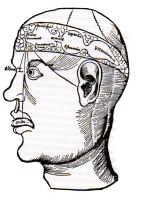
\includegraphics[width=0.2\textwidth]{./images/humoral.png}
\caption[From Gr\"{u}sser, 1990 \cite{grusser1990seat}]{A medieval diagram which shows how spirits were thought to flow and combine through the ventricles of the brain. Different ventricles were associated with different faculties, such as sensation and the ``common sense,'' integrating different senses, imagination, memory, and reason.}
\label{medieval}
\end{figure}

%Descartes?
During the Enlightenment, many speculated that connections between ideas in the mind are based on connections between fibers in the brain (neurons had not yet been identified as distinct structures.)\footnote{For more on this period of history, see Sutton (1998) \cite{sutton1998philosophy}. Sutton's discussion of Descartes is especially interesting, since it shows how Descartes had a connectionist styled account of the brain, which on his view  interacts with a non-physical soul via patterns of activity at the pineal gland. Other mechanist philosophers of the period such as Hobbes and La Mettrie had similar accounts but rejected the assumption of a non-physical soul.} In the 1700s, the empiricists Locke, Berkeley, and Hume famously claimed that ideas in the mind result from associations between simple sensory ideas: for example, a percept of an apple is composed out simple sensations corresponding to its color, shape, smell, and taste. One idea comes to mind, it calls another to mind, etc. Sometimes this happens instantaneously, as in the apple percept, but in other cases it might unfold in a temporal progression. Someone mentions apples, and that might make you think of fiber, which might in turn make you think of Raisin Bran. If someone mentions a person you know, associated thoughts about them--their age, where they live, their occupation, physical appearance, etc.--might also come to mind. One idea comes to mind, it calls another to mind, etc. Thus, the empiricists thought of the mind as something like an Interactive Activation and Competition (IAC) network (cf. Chapter \extref{ch_intro}) \cite{bain1873mind}.

In this period, David Hartley argued that the empiricist theory of associations could be explained by laws governing connected neurons \cite{hartley1834observations, bain1873mind}. For example, Hartley \cite{hartley1749observations} proposed that sensations $A,B,C,...$ which are associated with each other, are associated because of correlated associations between ``vibrations'' of brain fibers:
\begin{quotation}
PROPOSITION 10: Any sensations $A, B, C$, etc., by being associated with one another a sufficient number of times get such a  power over the corresponding ideas $a, b, c$ etc., that any one of the sensations $A$, when impressed alone, shall be able to excite in the mind $b, c,$ etc., the ideas of the rest.

PROPOSITION 11: Any vibrations $A, B, C,$ etc., by being associated with one another a sufficient number of times get such a  power over the corresponding miniature vibrations $a, b, c$ etc., that any one of the vibrations $A$, when excited alone, shall be able to excite in the mind $b, c$, etc. 
\end{quotation}
He proposed proposition 11 as a neural explanation of proposition 10, which is psychological. Note that proposition 11 is an early version of what would later became known as Hebb's rule or Hebbian learning (``neurons that fire together, wire together''), discussed below and in chapter \extref{ch_unsupervised}.

Later, in the 19th century, Bain illustrated these ideas with images that look strikingly like modern neural network diagrams, as in Fig. \ref{bain}.

\begin{figure}[h]
\centering
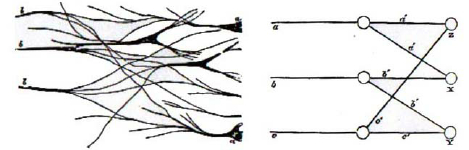
\includegraphics[scale=.7]{./images/bain.jpg}
\caption[From  \cite{bain1873mind}, pp. 110-111.]{From Bain's 1873 book \emph{Mind and Body}, which opens with the question ``What has Mind to do with brain substance, white and grey''?}
\label{bain}
\end{figure}

The notion that associations between thoughts and memories are based on neural connections in the brain was further developed in late 1800s by Sigmund Freud, who developed a psychodynamic theory, according to which  psychical ``energies'' are based on the flow of activations in the neural networks of the brain. His goal was to show how psychology could become a natural science by representing ``psychical processes as quantitatively determined states of specifiable material particles'' \cite[p. 355]{freud1954project}. But whereas earlier theorists had simply speculated about associative processes, he based his on actual  clinical observations, and in particular observations of (allegedly) neurotic patients experiencing ``excessively intense ideas.''  He explained his clinical observations in terms of ``neuronic excitation'' understood as ``quantities in a condition of flow'' (p. 356). Fig. \ref{freud} shows part of an image from this early book, which describes a patient (Emma Eckstein, who went on to become a famous author) who avoided shops based on an earlier traumatic experience. The specifics of the account are dubious, and Freud himself gave up on the project of a direct neural account of psychological processes,  but it does show that Freud was thinking about the mind in a broadly connectionist way.

\begin{figure}[h]
\centering
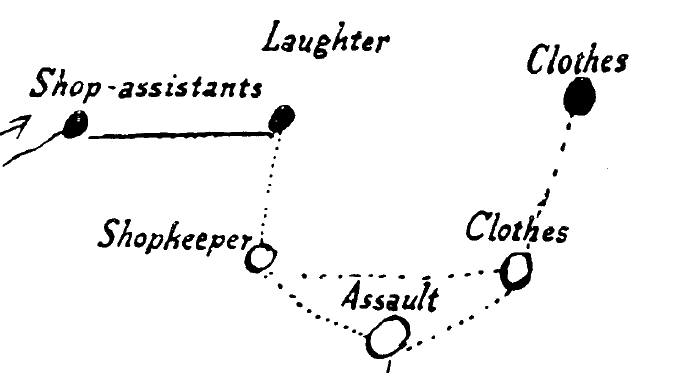
\includegraphics[width=0.5\textwidth]{images/freud_scientific_psychology.png}
\caption[From \cite{freud1954project}.]{An image from Freud's early \emph{Project for a Scientific Psychology}. The open circles are conscious ideas; the dark circles are unconscious ideas. }
\label{freud}
\end{figure}

Many other psychologists, neuroscientists, and philosophers in the late 19th and early 20th century contributed to the general idea that psychological processes are rooted in neural processes. Helmholtz, Mach, Ram{\'o}n y Cajal, Golgi, and others advanced biological psychology in various ways (see, e.g., \cite{boring1929history}), e.g. by establishing that neurons are individual cells, and by applying mathematical methods to psychology and neuroscience. In Russia, the psychologists Luria and Pavlov sought to understand the neural basis of associative learning, speech pathology, and other cognitive phenomena in a quantitative, experimentally tractable way.\footnote{On Luria in relation to the history of neural networks, see \cite[p. 41]{rumelhart1986parallel}.}

\section{Birth of Neural Networks}

We now turn to the history of neural networks proper, i.e. explicit formal descriptions of artificial neural networks, which could be implemented in computer programs.\footnote{The history of neural network research from this point forward is covered in several places. Fausett has a 4 page overview that covers the main points nicely:  \cite[pp. 22-26]{fausett1994fundamentals}. Levine, ch. 2 is especially detailed on McCulloch,s Pitts and Rosenblatt \cite{levine2000introduction}. A brief online history is at \url{http://cs.stanford.edu/people/eroberts/courses/soco/projects/neural-networks/History/}. A more recent history that extends to present day work in deep learning is at \url{https://www.skynettoday.com/overviews/neural-net-history}. Also see the end of chapter 1 of the first PDP chapter, \cite{rumelhart1986parallel}, and Haykin (2nd Ed.) section 1.9 \cite{haykin1998neural}. My favorite source is a series of interviews of leading figures in the history of neural networks collected in \emph{Talking Nets}, \cite{anderson2000talking}.} 

The first wave of research into neural networks occurred in the 1940s, via an array of neuroscientists, mathematicians, logicians, and engineers, many of them at MIT.\footnote{Important research relating to neural networks did occur earlier in the 20th century, e.g. work by Thorndike, Lashley, and Clark Hull. Hull's writings contain diagrams and formulas describing associative learning processes based on rat studies that look very much like connectionist networks (e.g. \url{http://psychclassics.yorku.ca/Hull/Hierarchy/part1.htm}).}   The history is complex, fascinating, and brimming with colorful personalities (see the early chapters of \cite{anderson2000talking}). This was the period when digital computers were first being developed by people like John von Neumann, a child prodigy who  later established a computer architecture still in use today (the ``von Neumann architecture''  \cite{von1981principles}). The architecture involves a separation between memory and a central processing unit that retrieves data from memory and operates on it using logical rules.
% Consider expanding the Hull discussion with a picture, esp. in light of the video

Neuroscience had also been steadily advancing in this period, and the network structure of the brain and its relation to behavior were better understood. The field of control theory was emerging via the work of Norbert Wiener, another child prodigy. He developed the field of ``cybernetics'' (which is closely related to modern control theory), and defined it as ``the science of control and communication in the animal and the machine'' \cite[p. 16]{wiener1948cybernetics}. In the late 1930s, the petroleum industry had developed central control systems to maintain refinery towers, and in WWII feedback systems were used to control anti-aircraft guns. A key idea in cybernetics was that these feedback circuits could coordinate complex movement, both in engineered systems and in the brain.

%  McCulloch: ``McCulloch was a psychiatrist and neuroanatomist by training: he spent some 20 years thinking about the representation of an event in the nervous system.
% Pitts. ```Pitt was a mathematical prodigy, who joined Mc Culloch in 1942.''
% They were logic oriented. Kleene had papers on this stuff. And these things emerged in the same literature as automata theory. Remember this is the beginning of formal logic and people realizing its potential.

In this atmosphere, two scientists emerged as the ``fathers of neural network theory'': Warren McCulloch (a neurophysiologist affiliated with cybernetics) and Walter Pitts (a logician).\footnote{Both had vivid personalities. McCulloch had wild hair and charisma. Pitts was a quiet introvert who had trouble getting a regular job, but who was regarded by his associates as a genius and was supported by McCulloch for many years. For a fascinating first-hand account of their personalities see the interviews with Lettvin, Cowan, and Arbib in \cite{anderson2000talking}. See in particular pages 9, 101, 104, 218, 223. Video interviews with McCulloch are available online.}  They wrote a famous paper  showing how neuron-like elements could perform all the logical operations performed by computers. This in turn implies that whatever can be done on a computer can, in principle, be done using neurons \cite{mcculloch1943logical}. A diagram from McCulloch and Pitt's famous paper, \emph{A Logical Calculus of Ideas Immanent in Nervous Activity}, is shown in figure \ref{mp}.\footnote{See Levine, p. 12, for a useful summary of how McCulloch / Pitts networks operate \cite{levine2000introduction}.}  In appendix \extref{ch_logicgates}, a demonstration of a similar approach to building logic gates using neural networks (in Simbrain) is developed.

\begin{figure}[h]
\centering
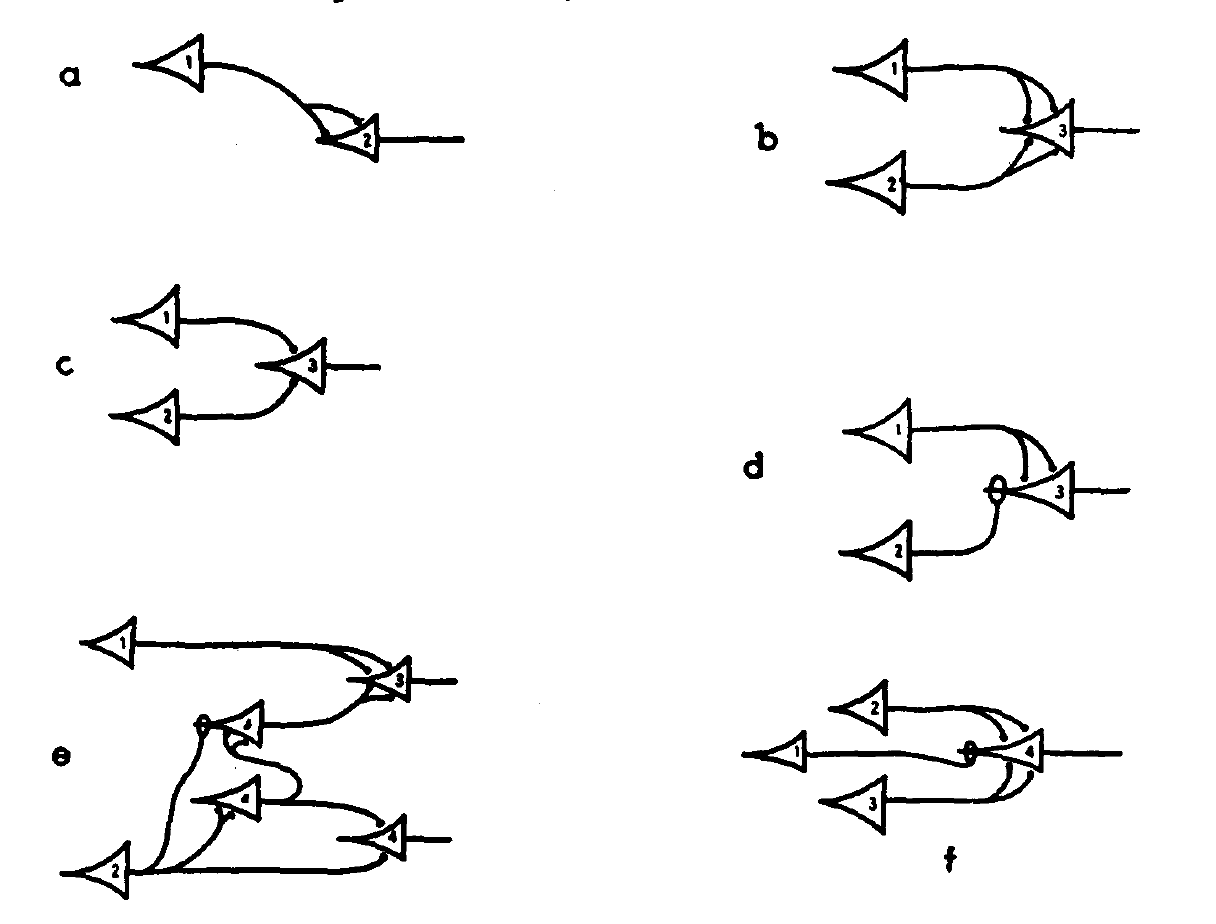
\includegraphics[width=0.5\textwidth]{./images/McCullochPitts.png}
\caption[From \cite{mcculloch1943logical}.]{From the end of McCulloch and Pitt's famous article, in which they demonstrate that ``for any logical expression satisfying certain conditions, one can find a net behaving in the fashion it describes.''  In these networks, what are today called ``weight strengths'' or ``synaptic efficacy'' correspond to number of connections. Nodes only fire if two or more incoming connections are activated. ``Lasso" connections correspond to what are today called ``inhibitory'' connections. In these networks, a single activated lasso connection will disable the node it is connected to. A network computing \emph{logical or} is shown in panel B (it will fire if either of the inputs nodes connected to it fires) and a network computing \emph{logical and} is shown in panel C (it only fires if both input nodes connected to it fire). Panel E models the heat illusion (briefly held cold objects can feel hot). For an elaboration of this case see \cite{piccinini2004first}.}
\label{mp}
\end{figure}
% Expand this. Explain the panel d is a connection with a shutoff. Insert a reference to a Simbrain model of the heat illusion and include text from the video.

McCulloch and Pitts used what are now called binary units or threshold units (see chapter \extref{ch_act_functions}): nodes that are only activated when their summed inputs are above a certain value. Nodes could only be active at a level of 0 or 1, based on the ``all or none'' property of neurons (cf. \extref{ch_neuro}). They made some assumptions that are unusual by today's standards. For example they assumed that a single inhibitory input is sufficient to completely prevent a neuron from firing. More importantly, they did \emph{not} describe connections between neurons using variable-strength weights. Their networks used fixed connections, which could not be adjusted using a learning rule. Learning rules would later become a  primary focus of neural network theorists. Nonetheless, it was the first time an actual formal model of a neuron was presented, together with a serious effort to understand how networks of neurons could produce complex behaviors.
% I think this is right, but check: \footnote{Though they did allow multiple connections between nodes, a multi-graph architecture not often used today.}

%Today neural networks are usually thought of in contrast to digital computers. In fact, in the introductory chapter \extref{ch_intro} we  opened by contrasting computation in a neural network with computation in a digital computer. But it is important to realize that this opposition came later. In this period people were just trying to figure out what a computer was. They were figuring out the mathematical underpinnings of computer science via the study of ``formal automata''. They knew the brain did some kind of computation and were interested in that. The neuroscientists were interested in what the logicians were doing. The engineers were interested in what the neuroscientists were doing. Etc. And in fact a neural network can implement a digital computer in principle. But in practice, the two styles of computation are distinct, and later on in the history the two approaches would be more strongly distinguished.

\section{The Cognitive Revolution}\label{cog_rev}

The next major event in the standard history of neural networks was the development of the \emph{Perceptron} in the late 1950s, which we discuss in the next section. However, during the 1950s-1970s many other developments took place that broadly supported a neural network approach to the study of cognition. Framing all these events was the emergence of cognitive science, via the ``cognitive revolution.''\footnote{An excellent overview and history of the era is \cite{baars1986cognitive}.}  Advances in linguistics, early computer science, neuroscience, and psychology, among others, coalesced in a broad reaction to earlier approaches to psychology, which had focused on observable behavioral data. These \emph{behaviorists} had frowned upon discussions of internal processing between sensory inputs and motor outputs, and treated the mind as a kind of black box. The emerging cognitive scientists wanted to break open that black box and look inside: they wanted to understand what kind of processing occurs between sensory input and motor output in terms of \emph{computation}. The big idea, the idea that got everyone excited, was that inside the mind there is an information processing system, one similar to the computer systems that were just then beginning to be realized on a large scale. 

%The cognitive revolution and some of the rifts that later developed within it are discussed in section \ref{philNeuralNets}. 

%This new breed of inter-disciplinary cognitive scientists would, however, split, according to \emph{how} they thought the mind processes information. Some thought (and some still think) that the mind processes information using symbols and rules, like a digital computer does. This remains a dominant tendency in cognitive science, and it goes by several names: ``functionalism'', ``Symbolic AI,'' and ``Classical AI'', among others. The other camp, the ``connectionists'', thought the mind processes information more like the brain does, by transforming patterns of activation using matrices of weights.\footnote{As noted above, it's interesting that McCulloch and Pitts (and von Neumann, father of the standard architecture for digital computers) did work before the ``AI/ Connectionism'' rift, showing that neurons could do anything a digital computer could do. }  Today there are other camps as well, and some who mix ideas from both symbolic AI and connectionism.
% Mix in some of that ai_nn stuff. This could be the place for developing those ideas...

Here are some themes in early cognitive science that prefigure connectionism. The Canadian psychologist and neuroscientist Donald Hebb formulated his famous learning rule for weights, the ``Hebb rule'' (``neurons that fire together, wire together'') \cite{hebb2005organization} (cf. the discussion of Hartley above).\footnote{See \url{http://www.scholarpedia.org/article/Donald_Olding_Hebb}. Also see Werbos' interview in  \cite{anderson2000talking}.}   Hebb also described the operation of the brain in terms of networks of connected neurons, formulating the concept of a ``cell assembly'', a group of neurons that becomes associated over time and thereafter tend to collectively reverberate in response to a stimulus (Fig. \ref{hebb} shows one of Hebb's own diagrams of a cell assembly) \cite{hebb2005organization}. The concept of a specific, learned pattern of brain activity produced by a stimulus remains important today.\footnote{See \url{http://www.scholarpedia.org/article/Cell_assemblies}. For a more up to date version of the idea cf. the concept of a polychronous neural group or PNG, \url{https://www.izhikevich.org/publications/spnet.htm}.}
% Need more information on the social network of Hebb. He does not seem too connected to the other figures.
% Some information in Haykin p. 38-39: ``Hebb's book was immensely influential among psychologists [like Anderson] but unfortunately it had little or no impact on the engineering community. Hebb's book [however] been the inspiration for the development of computational models of learning and adaptive systems" [Duda and Hart]   Uttley, leaky integrate and fire. 

\begin{figure}[h]
\centering
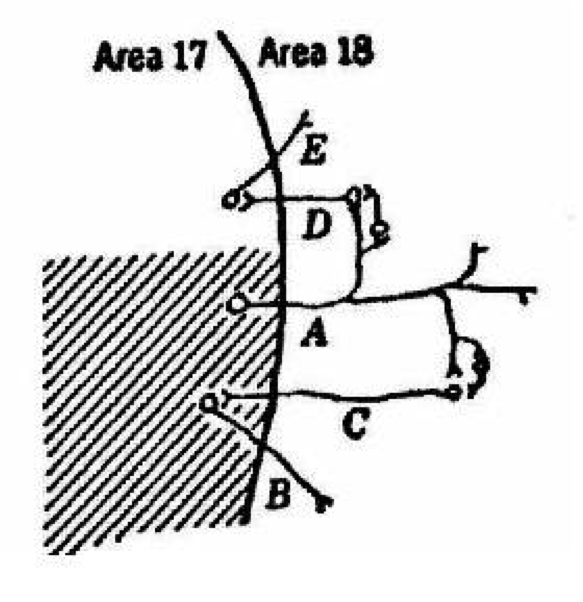
\includegraphics[width=0.4\textwidth]{./images/HebbCircuit.png}
\caption[From Hebb, 2005 \cite{hebb2005organization}]{A Hebbian cell assembly. These neurons initially fired together, and then got wired together, and so they will tend to fire together in the future.}
\label{hebb}
\end{figure}

\begin{figure}[h]
\centering
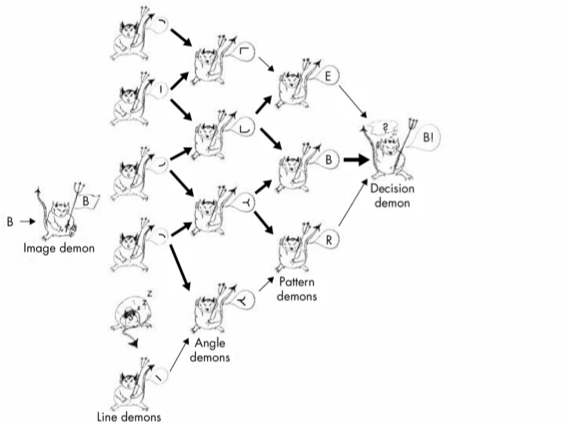
\includegraphics[width=0.5\textwidth]{./images/Selfridge.png}
\caption[From Groome, 2013 \cite{groome2013introduction}]{Selfridge's pandemonium model.}
\label{selfridge}
\end{figure}

Another important figure in the period was the psychologist Oliver Selfridge, who pioneered the idea that psychological processes can be broken down into interacting sub-processes. His ``Pandemonium'' theory described the mind as a collection of ``demons'', each of which takes care of one specific aspect of a task. For example, figure \ref{selfridge} shows how Selfridge thought of the process of perceiving the letter ``B''. An image arrives at the eye, line demons detect lines in various orientations, and those demons send messages to angle demons who detect angles, and the process continues through a network of demons until a decision demon says ``B!'' \cite{selfridge1958pandemonium}

%  Work here / add references
Other important research in this period was carried out by the psychiatrist and cyberneticist William Ashby (who wrote \emph{Design for a Brain} in 1952), Marvin Minsky (who wrote a dissertation on neural networks on 1954), and Dennis Gabor (a Nobel laureate who worked on holograms, and introduced a standard method for translating visual stimuli into a numeric form, that can be processed by neural networks).

\section{The Age of the Perceptron}

The types of layered feed-forward networks that  are typically used today were first studied in detail in the 1950s and 1960s, primarily via the work of Frank Rosenblatt and Bernie Widrow (both published seminal papers in the late 1950s and early 1960s; see \cite{widrow1960adaptive}).\footnote{A concise summary of this period of history is in Bishop p. 98 \cite{bishop1995neural}. Also see \cite{widrow1960adaptive}.}  Rosenblatt called his network the ``Perceptron'' and Widrow called his an ``Adaline''. Both had a single layer of adjustable weights, threshold output units, and learned using an error function (cf. Chap. \extref{ch_supervised}). Thus both networks moved beyond McCulloch and Pitt's networks to networks that actually learned from experience.\footnote{There were differences as well. The perceptron had separate layers of input nodes and fixed weights designed to help with visual classification tasks. The perceptron learned from a discrete on/off signal, while the Adaline learned from a continuous weighted input signal (a more modern way of doing things; cf. chapter \extref{ch_supervised}.) Widrow was an engineer who implemented the Adaline using a special electrical components called a ``memistor'' which Widrow designed himself.} 
% Use the crazy Skynet quote about what Rosenblatt thought his machines would achieve

\begin{figure}[h]
\centering
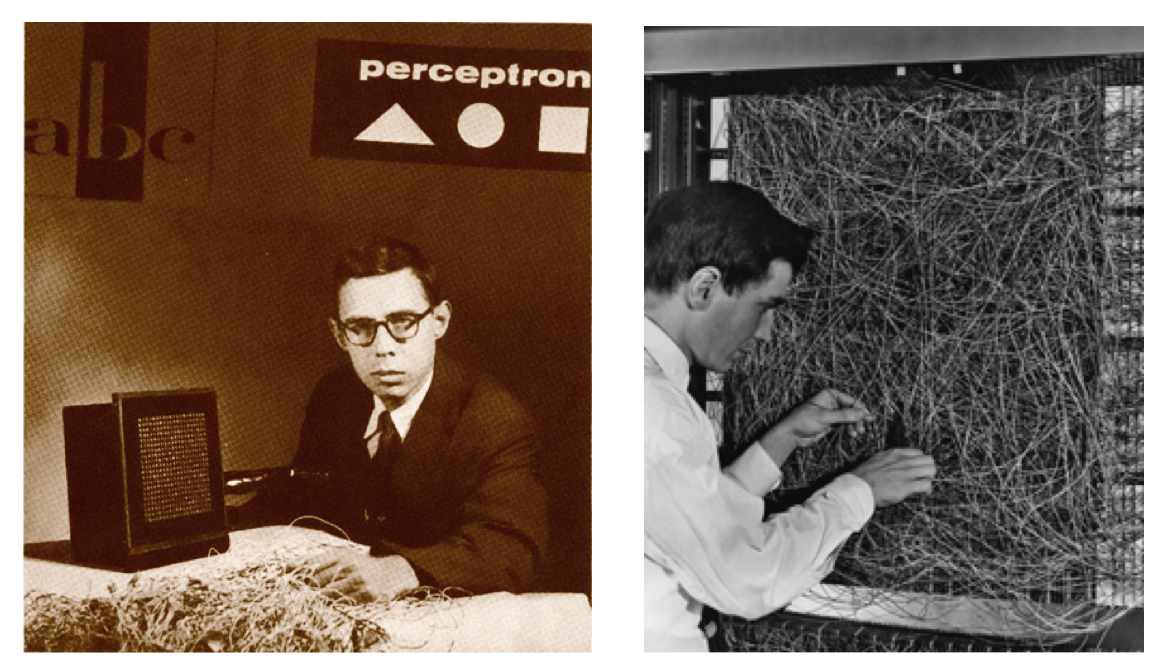
\includegraphics[width=0.7\textwidth]{images/perceptron.png}
\caption[Left: \url{http://www.rutherfordjournal.org/images/TAHC_rosenblatt-sepia.jpg}; Right: \url{http://www.newyorker.com/wp-content/uploads/2012/11/frank-rosenblatt-perception.jpg}]{Rosenblatt with one of his hardware implementations of a perceptron (left) and another view of the perceptron (right). }
\label{perceptron}
\end{figure}

Rosenblatt was a psychologist interested in human and animal behavior and its neural basis.\footnote{As with McCulloch and Pitts, Rosenblatt's personal history is fascinating, and in some ways tragic. See the Cowan and Hecht-Nielson interviews in Talking Nets \cite{anderson2000talking}.} He studied feed-forward networks with one layer of fixed weights and another layer of adjustable weights that could be trained to classify images on small displays as, for example, triangle vs. square, or male vs. female. He implemented his networks using huge tangles of wires for synaptic links (see Fig. \ref{perceptron}). This was quite impressive at the time and got a considerable amount of press.\footnote{See \url{https://www.youtube.com/watch?v=cNxadbrN_aI}} Rosenblatt also proved that perceptrons could find solutions to certain types of classification tasks in a finite time \cite{rosenblatt1962comparison}.\footnote{This is known as the ``perceptron convergence theorem.''} Haykin, who refers to this as the ``classical period of the perceptron'', summarizes Rosenblatt's importance as follows:
\begin{quotation}
The perceptron occupies a special place in the historical development of neural networks: It was the first algorithmically described neural network. Its invention by Rosenblatt, a psychologist, inspired engineers, physicists, and mathematicians alike to devote their research effort to different aspects of neural networks in the 1960s and the 1970s. Moreover, it is truly remarkable to find that the perceptron... is as valid today as it was in 1958 when Rosenblatt's paper on the perceptron was first published.
\end{quotation}

Whereas Rosenblatt focused on psychological implications of the perceptron, Widrow and his colleagues had engineering applications in mind, like adaptive noise cancelling in telephone wires.\footnote{According to Widrow this technology is used in every modem in the world and is at the heart of the internet; see \url{https://www.youtube.com/watch?v=skfNlwEbqck} which also shows him demonstrating his old hardware Adaline.} In the hardware implementation shown in Fig. \ref{adaline}, the toggle switches control input node activations, the knobs control weight strengths, and the dial shows the activation of an output node.\footnote{For Widrow's personal recounting of the Adaline and its history, see his interview in \emph{Talking Nets} \cite{anderson2000talking}. Also see the videos referenced in the Figure caption.}
% Improve the discussion above, referring to the mathematical improvements in the delta rule / Adaline, and also refer forward to \extref{ch_supervised_ff}, which has a discussion of these changes and a footnote on that part of the history.

\begin{figure}[h]
\centering
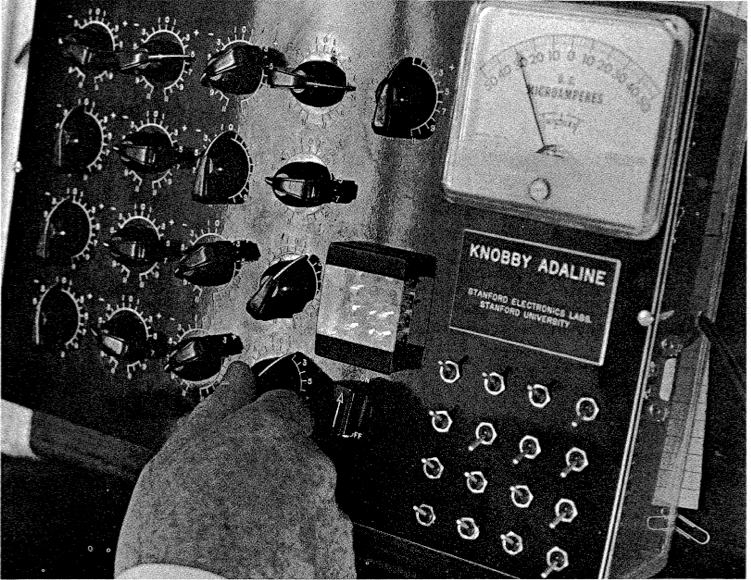
\includegraphics[scale=.3]{./images/adaline.png}
\caption[From \cite{widrow1963adaline}.]{A hardware implementation of Widrow and Hoff's ``Adaline'' network, which Widrow called the ``knobby Adaline'' on account of the prominent grid of knobs on the left, which control weight strengths, and which were manually adjusted to implement their learning algorithm. Inputs were produced using the 12 toggle switches on the lower right (and displayed in the grid of small lights), and the resulting output activation is displayed in the meter on the upper right. Videos of Widrow demonstrating the knobby Adaline, back in the 60s and also more recently, are available at \url{https://www.youtube.com/watch?v=skfNlwEbqck} and \url{https://www.youtube.com/watch?v=IEFRtz68m-8&t=161s}.}
\label{adaline}
\end{figure}

\section{The ``Dark Ages''}\label{dark_ages}

% Haykin points out the issues were part psychological, part financial. And other stuff. See p. 40
% Mention the convergence theorem itself
% Neocognitron, which anticipates deep learning. Done in industry. It's also a lot like pandemonium
% Sharai - We need references for Kohonen, Anderson, Braitenberg, Grossberg, and Carpenter.
% More on RL

Perceptrons and Adalines created a surge of interest in neural networks in the 1960s, but this was followed by a period of relative quiescence in the 1970s and 1980s, during what have been called the ``dark ages'', ``quiet years'', ``drought'', and ``winter'' of neural networks.\footnote{See PDP vol 1, ch. 1 \cite{rumelhart1986parallel}; Haykin p. 43 \cite{haykin1998neural}; Fausett p. 24 \cite{fausett1994fundamentals}. A variety of perspectives on the period are discussed in Talking Nets. 110, 155, 254, 305, 371. Grossberg, Carpenter, Kohonen, Anderson and others active in this period have their own interviews in Talking Nets \cite{anderson2000talking}.}  The dropoff in interest has been attributed to several causes. The canonical story is that networks with a single layer of adjustable weights were shown by Minsky and Papert to suffer certain fundamental limitations \cite{minsky1969perceptrons} (cf. Chap. \extref{ch_supervised}). So it was thought that neural networks weren't powerful enough to do psychologically realistic things. Moreover, at precisely that time more symbolic AI models were flourishing. 

However, even if interest in neural networks waned for a time, especially in comparison to AI, neural network research was active in this period. Relevant researchers include Kohonen, Fukushima, Anderson, Sutton, Barto, Braitenberg, Grossberg, and Carpenter. These and others laid the foundations for many of the ideas described in this book. So the dark years really weren't that dark.\footnote{Debates about the the status of neural networks in this period are covered in some detail in Talking Nets \cite{anderson2000talking}.} 
% Mention that Fukushima worked on early deep networks. Say a bit about the others too, at least in a footnote

\section{First Resurgence: Backprop and The PDP Group}

% This section needs to be enhanced. This is where we get the cog-sci stuff. It's what the book is suppsoed to be about. Refer back to Bain and Freud's hopes. This flashes by currently. OR at least refer back to the material in ch. 1 which does some of the work.

% See the connectionists email about the history of backprop, and all the discussion in talking nets. Clearly Werbos should be discussed, but there were others too.
% Sharai - We need a reference for the discovery of backpropagation algorithm (is discovery in reference to it's creation or it's first application in neural networks?).
Connectionism came out of its (allegedly) dark decade and enjoyed a resurgence in the 1980s, for several reasons, including the discovery of the backpropagation algorithm, which overcomes the limitations associated with perceptrons. While neural networks were being shown to be more powerful than had previously been thought, the competing program of symbolic AI was running into problems \cite{dreyfus1992computers}. 

Another reason for this renewed interest---particularly among cognitive scientists---was the publication of a major two-volume work in the period, {\em Parallel Distributed Processing: Adventures in the Microstructure of Cognition}, in 1986, by David Rumelhart, James MClelland, and the ``PDP research group'' (a group of researchers, many of whom were at UC San Diego.)  This publication brought connectionist networks back to the forefront, by clearly articulating the connectionist standpoint, showcasing a number of models of various aspects of cognition, and clarifying how connectionist networks differ from symbolic AI models \cite{rumelhart1986parallel}. John Hopfield's models of associative learning in recurrent networks (i.e. ``Hopfield nets'', discussed in chapter \extref{ch_unsupervised}) were also influential in this period, in part because Hopfield presented his work in an especially clear, mathematically precise way.\cite{hopfield1982neural}.\footnote{In Talking nets, on the PDP group, see pp. 180, 254, 277, and 281. On  backprop and its history, see 286, 327, and 338. On Hopfield, see 113, 301 \cite{anderson2000talking}.}

% Net-talk was huge. See Talking Nets 324. I have material on this for other classes. Also Sejnowski is an important figure and should be mentioned.

\section{Second Decline and Second Resurgence: The Deep Learning Revolution}

% Rename to "A new winter and its thaw" and cite sknet paper?
% There must be cool things to link to here for deep learning, e.g. a distll.pub interactive article

% Add reference to data science book that describes this sentiment. Maybe also that automatic diff video
For a time (roughly the late 1990s through about 2010), neural networks declined in interest as attention shifted to machine learning algorithms (cf. chapter \extref{ch_intro}). The problem was, in part, that tuning the parameters of a neural network seemed more an art than a science, especially when compared with machine learning, which is based on more tractable statistical principles. There was a sense that people just ``twiddled''  the knobs of a simulation as best they could until they got decent performance out of their network. In 2010, Phillip Jannert clearly expressed this concept of a second decline: ``Neural networks were very popular for a while but have recently fallen out of favor somewhat. One reason is that the calculations required are more complicated than for other classifiers; another is that the whole concept is very \emph{ad hoc} and lacks a solid theoretical grounding'' \cite[Ch. 18]{janert2010data}.
% The skynet discussion of this useful. "But, this did little to fix the larger perception problem that neural nets were janky and did not work very well. They were seen as a hassle to work with - the computers were not fast enough, the algorithms were not smart enough, and people were not happy." [from skynet]

% More on deep learning, and perhaps a glossary item. Clarify that deep learning is just one kind of NN used in deep learning.
However, several things happened that have brought attention back to neural networks : (1) larger datasets for training neural networks have become available (hence current interest in ``big data''), (2) higher performance hardware for parallel neural network computing has emerged, for example by using the graphical processing units or GPUs on graphics cards (the kinds used to play modern graphics intensive video games) and in proprietary hardware such as Google's tensor processing units (TMUs),\footnote{It is interesting that these games require lots of parallel processors to render texture and shading in real-time graphics processing using linear algebra (cf. chapter \extref{ch_linear_algebra}), and that the same parallel processing circuits can be used to run neural networks. When graphics cards were first developed they did not have neural networks in mind!} (3) new neural network architectures have emerged, and (4) more principled ways of training networks have been developed that provide the area with improved  theoretical grounding, e.g. via ``Bayesian hyperparameter optimization.''\footnote{On moving beyond parameter ``tweaking'' or ``fiddling'' to more systematical methods, see the first 6 minutes of this video \url{https://www.youtube.com/watch?v=sq2gPzlrM0g}.}

% Expand this
Whereas most neural networks through the 1990s were just three layers, newer \emph{deep learning} architectures can have many layers of units. These many-layered deep-learning networks existed as far back as the 1970s, but it is only in the 2010s  that a variety of technical hurdles relating to this type of network were surmounted. Indeed many have described the period since the 2010s as a deep learning revolution, or as the decade of deep learning.\footnote{Andrey Kurenkov's history (\url{https://www.skynettoday.com/overviews/neural-net-history}) is excellent on these points. The achievements since 2010 are too numerous to survey here, but see \url{https://bmk.sh/2019/12/31/The-Decade-of-Deep-Learning/}} 